\chapter{Evaluation}
\label{cap:cap05}

In this chapter we evaluate our work in terms of the requisites presented on section \ref{sec:sec02}. The first section shows in numbers how many features are covered by the software switch. Subsequently, in the next section, we present the results of performance benchmarks tests. The last section of the chapter is a qualitative evaluation about the code's ease to change. We demonstrate the code portability, highlighting the port of the software switch to another processor architecture in a different operating system.      

The software switch evaluated version dates from the last commit pushed to GitHub. The box below shows the dates and last code changes description.

\begin{framed}

\begin{itemize}
\item \textbf{commit} cb740bd2565ac7e5d61ebe30ee75160a5452a033
\item   \textbf{Commit:}     Eder Leão Fernandes <ederleaofernandes@gmail.com> 
\item \textbf{CommitDate:} Mon Feb 23 18:42:49 2015 -0300 
\end{itemize}
     
    Add flags member to ofp_flow_stats.
    
    Fix missing flags field in the response of a flow stats request.
\end{framed}

\section{Feature Completeness}
\label{sec:FeatureComplete}
Evaluating the proper operation of the OpenFlow switch features is not a trivial task. This is caused by the multiple and rich configurations allowed by the specification. For example, testing all flow match fields combinations would require creation of a large number of flows and packets, making manual tests very time consuming. For this reason, automatic test frameworks, discussed on section \ref{sec:testemulation}, are the best options to test the switch functionality in order to evaluate feature completeness.    

OFTest and Ryu Certification are the two test frameworks used for the switch validation. As mentioned in chapter \ref{CodeMaintenance}, both are important tools for the software switch development. While Ryu certification has a strong focus on validation of the Datapath, OFTest offers a nice set of test cases for control and data plane message exchange. In the next sections we present a resume of the results obtained.  


\subsection{OFTest results}

Testing in OFTest is simple as it provides scripts in Python to run the switch and the test cases. Each test case starts a controller which connects with a running switch, executes the test instructions and checks the switch answers. 

Some messages from controller to switch, like a \textit{flow stats} request, and symmetric messages demand an answer from the switch. Thus, the main purpose of the framework usage with the software switch is for message handling validation. Although OFTest has capabilities to evaluate the pipeline processing - for instance, checking if a packet was correctly forwarded by a flow - we found in Ryu a more comprehensive test set for this task. 

Table \ref{tab:oftestbasic} shows test results for basic OpenFlow messages. The major type of messages of the test set are messages to query information about the state of manifold switch elements, such as \textit{GroupFeatureStats} and \textit{MeterStats}. Also, there are some configuration messages, like the \textit{PortConfigMod}. In all tests the switch returned the right answer for the control plane.


\begin{table}[h]
\centering
\caption{Basic OpenFlow messages}
\label{tab:oftestbasic}
\begin{tabular}{|l|l|l|l|l|}
\cline{1-2} \cline{4-5}
\multicolumn{1}{|c|}{\textbf{Message}} & \textbf{Result} &  & \textbf{Message}   & \textbf{Result} \\ \cline{1-2} \cline{4-5} 
AggregateStats                         & ok              &  & GroupFeaturesStats & ok              \\ \cline{1-2} \cline{4-5} 
AsyncConfigGet                         & ok              &  & GroupStats         & ok              \\ \cline{1-2} \cline{4-5} 
DescStats                              & ok              &  & MeterConfigStats   & ok              \\ \cline{1-2} \cline{4-5} 
Echo                                   & ok              &  & MeterFeaturesStats & ok              \\ \cline{1-2} \cline{4-5} 
EchoWithData                           & ok              &  & MeterStats         & ok              \\ \cline{1-2} \cline{4-5} 
FeaturesRequest                        & ok              &  & QueueStats         & ok              \\ \cline{1-2} \cline{4-5} 
FlowStats                              & ok              &  & PortConfigMod      & ok              \\ \cline{1-2} \cline{4-5} 
FlowRemoveAll                          & ok              &  & PortDescStats      & ok              \\ \cline{1-2} \cline{4-5} 
GroupDescStats                         & ok              &  & TableStats         & ok              \\ \cline{1-2} \cline{4-5} 
\end{tabular}
\end{table}

Controller roles test results are shown in table \ref{tab:oftestrole}. These tests check if the software switch changes correctly controller roles, and if the respective permission police is respected. As in the previous message tests, all role tests were successful.    

\begin{table}[h]
\centering
\caption{Role request message results}
\label{tab:oftestrole}
\begin{tabular}{|l|l|}
\hline
\textbf{Role Request Tests} & \textbf{Results} \\ \hline
RoleRequestEqualToSlave     & ok               \\ \hline
RoleRequestSlaveToMaster    & ok               \\ \hline
RolePermissions             & ok               \\ \hline
RoleRequestEqualToMaster    & ok               \\ \hline
RoleRequestNochange         & ok               \\ \hline
SlaveNoPacketIn             & ok               \\ \hline
\end{tabular}
\end{table}

\subsection{Ryu Certification results}

The Ryu Certification tests are divided into five categories: Action, Set-Field, Match, Group and Meter. The test sets of each category are very comprehensive, with tests for different packet types.

Table \ref{tab:ryuresults} is a resume of test results - the complete list of test cases can be found on Annex \ref{annex:ryucert} - for this work compared to the other three switches presented on chapter \ref{cap:cap02}. White cells give the number of tests passed, while grey cells show the number of test cases that returned an error. Tests are divided by each category, with the last two columns giving the total sum of working and non working features. The first row presents the results for this work. \footnote{ofsoftswitch13 is the software switch repository name} 

% Please add the following required packages to your document preamble:
% \usepackage{graphicx}
% \usepackage[table,xcdraw]{xcolor}
% If you use beamer only pass "xcolor=table" option, i.e. \documentclass[xcolor=table]{beamer}
\begin{table}[h]
\centering
\caption{Ryu Certification results comparison}
\resizebox{\textwidth}{!}{%
\begin{tabular}{|l|ll|ll|ll|ll|ll|ll|}
\hline
\textbf{Switch}       & \multicolumn{2}{l|}{\textbf{Action}} & \multicolumn{2}{l|}{\textbf{Set-Field}} & \multicolumn{2}{l|}{\textbf{Match}} & \multicolumn{2}{l|}{\textbf{Group}} & \multicolumn{2}{l|}{\textbf{Meter}} & \multicolumn{2}{l|}{\textbf{Total}} \\ \hline
\textbf{ofsoftswitch13} & 50    & \cellcolor[HTML]{9B9B9B}6    & 159    & \cellcolor[HTML]{9B9B9B}7      & 708  & \cellcolor[HTML]{9B9B9B}6    & 15   & \cellcolor[HTML]{9B9B9B}0    & 30   & \cellcolor[HTML]{9B9B9B}6    & 848  & \cellcolor[HTML]{9B9B9B}25   \\ \hline
\textbf{Open vSwitch} & 34    & \cellcolor[HTML]{9B9B9B}22   & 96     & \cellcolor[HTML]{9B9B9B}74     & 534  & \cellcolor[HTML]{9B9B9B}180  & 0    & \cellcolor[HTML]{9B9B9B}36   & 0    & \cellcolor[HTML]{9B9B9B}36   & 670  & \cellcolor[HTML]{9B9B9B}321  \\ \hline
\textbf{LINC}         & 24    & \cellcolor[HTML]{9B9B9B}32   & 68     & \cellcolor[HTML]{9B9B9B}102    & 428  & \cellcolor[HTML]{9B9B9B}286  & 3    & \cellcolor[HTML]{9B9B9B}12   & 0    & \cellcolor[HTML]{9B9B9B}24   & 523  & \cellcolor[HTML]{9B9B9B}456  \\ \hline
\textbf{Trema}        & 50    & \cellcolor[HTML]{9B9B9B}6    & 159    & \cellcolor[HTML]{9B9B9B}11     & 708  & \cellcolor[HTML]{9B9B9B}6    & 15   & \cellcolor[HTML]{9B9B9B}0    & 34   & \cellcolor[HTML]{9B9B9B}2    & 852  & \cellcolor[HTML]{9B9B9B}25   \\ \hline
\end{tabular}
}
\label{tab:ryuresults}
\end{table}

Results show that the software switch has a higher number of working features than Open vSwitch and LINC. With only 25 errors, it is tied with Trema in the number of supported features. There is a small difference between ofsoftswitch13 and Trema in the total number of tests passing. This happens because Ryu Certification does not execute four tests due to old switch restrictions.

The values presented in this section are from the official certification site. Some failed test results are presented on the site work in our internal test setup. For instance, matching on \textit{PBB ISID} value works as expected when tested in our development machine. However, we chose to show the official results as we could not identify the reasons for different results. In addition, some test may never pass. For example, \textit{IP proto} modification causes packet malformation, because the IP proto packet field will not conform with the next layer protocol, which leads to a test failure. 

\section{Performance Benchmarks}

One of the software switch requirements listed on chapter \ref{cap:intro} is to reach a maximum throughput of at least 100 Mb/s. For this reason we evaluated the switch performance in terms of network metrics. In this section we show how the switch performs for different packet sizes in comparison with the userspace switches LINC and Trema. We do not compare with OVS, since it is a software switch for production networks. Also, we investigated how performance is affected by the number of flows and by the number of tables traversed to match a packet.  

The machine configuration used to perform measurement tests are listed in the box below. 

\begin{framed}

\begin{itemize}
\item \textbf{Processor}:	8x Intel(R) Core(TM) i7-2670QM CPU @ 2.20GHz
\item \textbf{Memory}:	6003MB 
\item \textbf{Operating}: System	Ubuntu 14.04.2 LTS
\end{itemize}

\end{framed}

    \subsection{Maximum Throughput}
    \label{sec:MaxBand}
    This test evaluates the maximum forwarding rate the software switch can reach in comparison to other userspace implementations. 
    
    The setup for maximum throughput evaluation is the following:
    
    \begin{itemize}
    \item A running instance of the software switch with two virtual interfaces - Port 1 and Port 2 - attached. 
    \item One flow installed in the Flow Table to match a packet sent to Port 1 with destiny ethernet 00:00:00:00:01. The action is an output packet to Port 2. 
    \item A packet traffic generator. We used a simple program named packeth \cite{packeth}.
    \item A script running in the Linux terminal checking the current packet rate on Port 2.   
    \end{itemize}
    
    The test starts by installing the flow in the switch Flow Table. Afterwards, we inject packets, using the traffic generator, directly into Port 1. The bandwidth results of Port 2, reported by the script, are used to calculate the average rate and the standard deviation.  
    Two transmission measurements were made: for small packets of 64Kb and bigger packets of 1500Kb. Figure \ref{graph:comparison} shows results for both experiments.

    \begin{figure}[H]
        \begin{minipage}{\textwidth}
        \centering
        \begin{subfigure}{.7\textwidth}
        \begin{tikzpicture}    
 
         \begin{axis}[
            xtick=data,
            symbolic x coords={ofsoftswitch13, LINC, Trema},
            nodes near coords,
            width= 10cm,
            bar width=1.5cm,
            enlarge x limits={abs=1.2cm},
            ylabel near ticks,
            xlabel near ticks,
            ymin=0,
            ylabel=Throughput (Kpps),
            visualization depends on=-y \as \negy,
            visualization depends on=y \as \y,
            visualization depends on=\thisrow{error} \as \yerror,
            every node near coord/.append style={
                font=\small,
                shift={(0, transformdirectiony(\negy))},
                text width=1.5cm,
                align=center
            },
            nodes near coords={\pgfmathprintnumber{\y} $\pm$ \pgfmathprintnumber[fixed,precision=4]{\yerror}}]
        
        \addplot[ybar,fill=lightgray,error bars/.cd,y dir=both, y explicit]
        table[y error=error] {
            x y error
            {ofsoftswitch13} 38.08 0.17
            {LINC} 26.13 0.18
            {Trema} 166.42 26.57
        };
        \end{axis}
            
         \end{tikzpicture}
            \caption{Comparison using packets of 64 bytes}
            \label{graph:comparison64}
        \end{subfigure}
        \linebreak
        \begin{subfigure}{.7\textwidth}
        \begin{tikzpicture} 
        
          \begin{axis}[
            xtick=data,
            symbolic x coords={ofsoftswitch13, LINC, Trema},
            nodes near coords,
            width= 10cm,
            bar width=1.5cm,
            enlarge x limits={abs=1.2cm},
            ylabel near ticks,
            xlabel near ticks,
            ymin=0,
            ylabel=Throughput (Mbps),
            visualization depends on=-y \as \negy,
            visualization depends on=y \as \y,
            visualization depends on=\thisrow{error} \as \yerror,
            every node near coord/.append style={
                font=\small,
                shift={(0, transformdirectiony(\negy))},
                text width=1.5cm,
                align=center
            },
            nodes near coords={\pgfmathprintnumber{\y} $\pm$ \pgfmathprintnumber[fixed,precision=4]{\yerror}}]
        
        \addplot[ybar,fill=lightgray,error bars/.cd,y dir=both, y explicit]
        table[y error=error] {
            x y error
            {ofsoftswitch13} 260.25 1.67
            {LINC} 280.35 14.18
            {Trema} 843.56 17.70
        };
        \end{axis}
        
        \end{tikzpicture}
            \caption{Comparison using packets of 1500 bytes}
            \label{graph:comparison1500}
        \end{subfigure}
        \end{minipage}
        \caption{User space software switches throughput comparison}
        \label{graph:comparison}
    \end{figure}
  
   Switch forwarding performance for small packets is evaluated in Kilo packets per second (Kpps). Figure \ref{graph:comparison64} shows that ofsoftswitch13 can handle 38.08 Kpps. This result is very 
   far from Trema and approximatelly 32\% more efficient than LINC. Bigger packets are measured in Megabits per second. Results presented in Figure \ref{graph:comparison1500} show that ofsoftswitch13 and LINC, with rates of 260.25 Mbps 280.35 Mbps respectively, are slower than Trema with a bandwidth of 843.56 Mbps. 
   
    Although Trema overcomes our work in throughput performance, due to optimizations like multiple threads, the most important result of this experiment is the software switch maximum throughput found. This value is higher than the value established by the software switch requirements. 
    
    \subsection{Throughput in function of flows and tables}
    \label{sec:bandflows}
    This experiment measured two factors that may affect the software switch performance. One is the number of flows installed in one table. The second is the number of tables traversed until the match is found.
    
    For this test we used Mininet with the software switch connecting two hosts. Bandwidth is measured through the  Iperf session established between the two hosts. Flow Table setup for the two cases are the following: 
    
    \begin{enumerate}[label=(\Alph*)]
    \item \textbf{Number of flows}. A certain amount of flows, with the same priority, that will not match packets is installed. In the end, two flows, with the same or lesser priority than the previous, are installed to forward packets between the two hosts.
    \item \textbf{Number of tables}. Flows to send the packet to next table are installed until the penultimate table. Then, in the last table two flows are added to forward the traffic between the hosts.
    \end{enumerate}
    
        \begin{figure}[h!]
            \begin{minipage}[b]{\textwidth}
            \centering
        \begin{subfigure}[b]{.5\textwidth}
            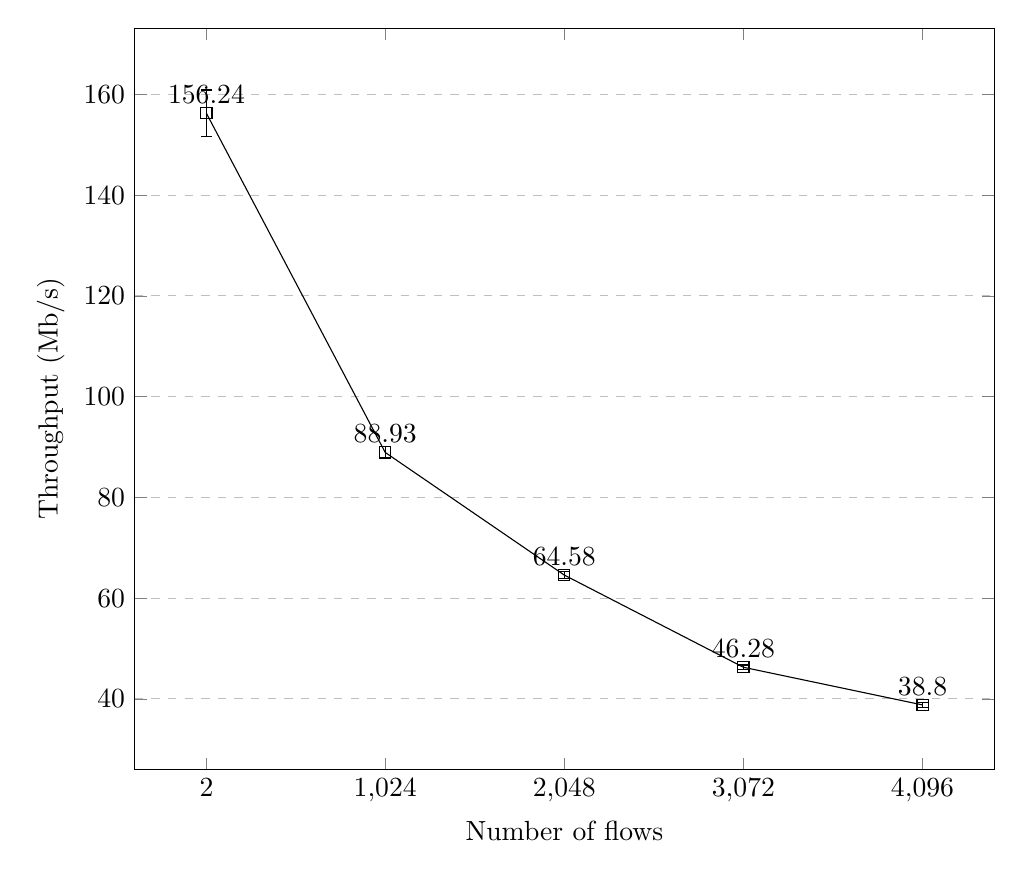
\begin{tikzpicture}
            \begin{axis}[
                xlabel={Number of flows},
                ylabel={Throughput (Mb/s)},
                ymajorgrids=true,
                grid style=dashed,
                ylabel near ticks,
                nodes near coords,
                scale only axis,       
                width=.9\textwidth,
                xlabel near ticks,
                xtick={2, 1024, 2048, 3072, 4096},
            ]
            \addplot[color=black, mark=square,error bars/.cd,y dir=both, y explicit]
            coordinates {
                (2, 156.24) +- (0.00, 4.64709)
                (1024, 88.93) +- (0.00, 1.20467)
                (2048, 64.58) +- (0.00, 0.65115)
                (3072, 46.28) +- (0.00, 0.4492)
                (4096, 38.8) +- (0.00, 0.52493)
            };
            \end{axis}
            \end{tikzpicture}
            \caption{Throughput per number of flows in one table}
            \label{graph:nflows}
        \end{subfigure}
         \hfill
        \begin{subfigure}[b]{.5\textwidth}
            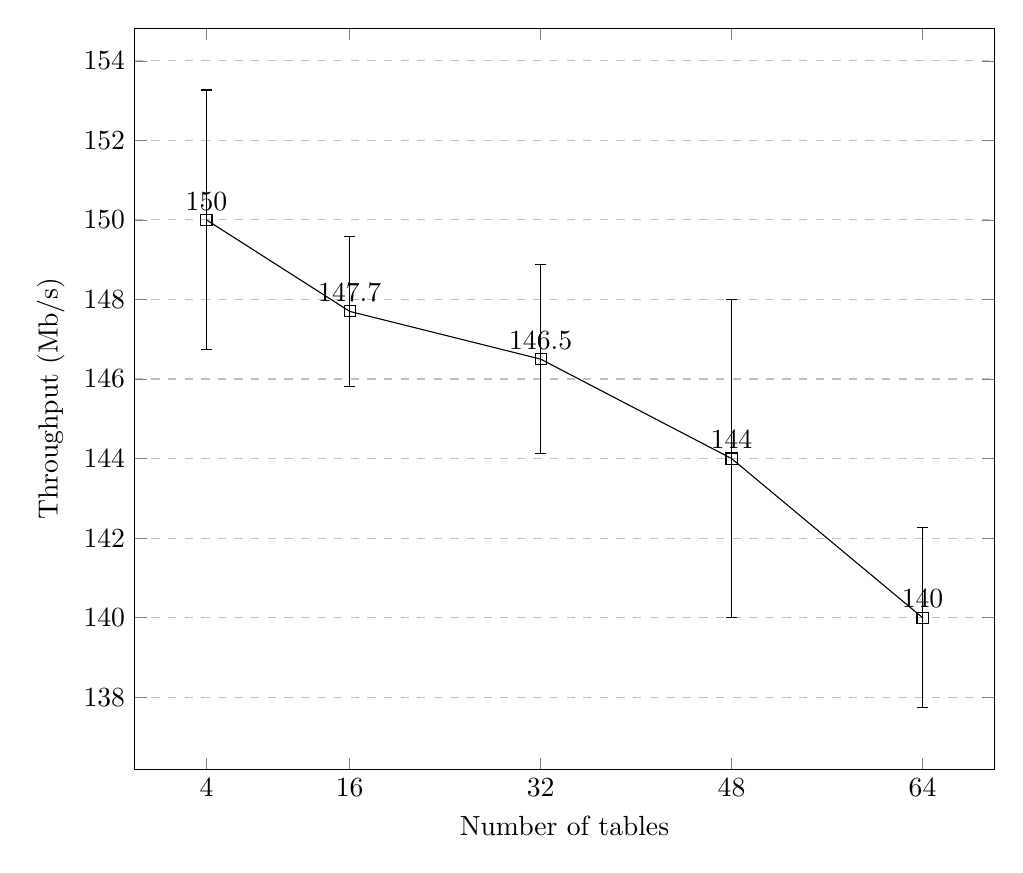
\begin{tikzpicture}
            \begin{axis}[
                xlabel={Number of tables},
                ylabel={Throughput (Mb/s)},
                ymajorgrids=true,
                grid style=dashed,
                ylabel near ticks,
                nodes near coords,
                scale only axis,       
                width=.9\textwidth,
                xlabel near ticks,
                xtick={4, 16, 48, 32, 64},
            ]
            \addplot[color=black, mark=square,error bars/.cd,y dir=both, y explicit]
            coordinates {
                (4, 150) +- (0.00, 3.26599)
                (16, 147.7) +- (0.00, 1.88856)
                (32, 146.5) +- (0.00, 2.36878)
                (48, 144)   +- (0.00, 4)
                (64, 140) +- (0.00, 2.26078)
            };
            \end{axis}
            \end{tikzpicture}
            \caption{Throughput per number of tables}
            \label{graph:ntables}
        \end{subfigure}
        \end{minipage}
            \caption{Influence of the number of installed flows on the throughput.}
            \label{graph:scaling}
        \end{figure}     
     
        The graphs in the Figure \ref{graph:scaling} shows that both cases have a strong influence over the switch performance. The most sensitive case is for one table shown in Figure \ref{graph:nflows}, as the number of flows increases the throughput decreases linearly. The increase in the number of tables, shown by the graph in the Figure \ref{graph:ntables}, also causes a linear decrease in the packet rate, though it is smaller than in the first case. These results were expected, since the software switch implements linear matching. Thus, this experiments were important to verify one improvement area for the software switch.     
     
    \subsection{Ping Round Trip Time}

    Round Trip Time (RTT) is the time between a data request and answer. Several factors might affect the total RTT and  influence network's latency. Two examples are: the number of nodes between two communicating hosts and the transmission medium. The time a packet takes to enter and leave a switch is also considered for the RTT. Thus, it is important to measure how much the software switch affects the RTT. 
    
    In order to measure the RTT between two hosts connected by our software switch - we also compare LINC and Trema -, the following steps are executed:
    
    \begin{enumerate}
    \item Creation of two Linux containers (LXC) - Host 1 and Host 2 - with a pair of virtual interfaces \textit{veth0} and \textit{veth1}. LXC is an operating system lightweight virtualization technology, in which it is possible to run multiple isolated Linux instances as containers. With LXC, we run two containers to serve as the network hosts.    
    \item Execution of a software switch instance with the container virtual ports attached to switch interfaces.
    \item Installation of two flows in the switch Flow Table to forward the traffic between the two hosts. 
    \item Configuration of Host 1 and Host 2 with IP addresses in the same network. In our test Host 1 is configured with the IP address 192.168.0.1 and host 2 as 192.168.0.2. 
    \item Execution of the \textit{ping} program in Host 1 to ping the address 192.168.0.2. Ping is a program to send and measure the time between an Internet Control Message Protocol (ICMP) "Echo request" and the ICMP "Echo Reply". The number of Echo requests sent is 100 and the packet sizes are 64Kb.
    \end{enumerate}

    Switch results comparison is shown in Table \ref{pingtable}. These tests give a good approximation for the software switch impact over the network delay, because it is connected directly to the hosts. As expected, because of the previous results, Trema is the most efficient among the userspace software switches. The ofsoftswitch13 obtains a low minimum RTT, with 0.304 ms, compared to the average of approximately 1ms. LINC has a very high RTT, with more than a half second to complete. This is not a surprise, because the throughput tests, shown in section \ref{sec:MaxBand}, revealed that LINC does not handle small packets efficiently.
    
    An acceptable RTT value depends on the application running over the network. Latency sensitive programs, like multiplayer online games, benefit from a low RTT. Considering a small network, with not many hops, the RTT in our software switch is acceptable.   

        % Please add the following required packages to your document preamble:
    % \usepackage{graphicx}
    \begin{table}[H]
    \caption{Ping Round Trip Time comparison between software switches}
    \label{pingtable}
    \resizebox{\textwidth}{!}{%
    \begin{tabular}{|l|c|l|c|c|}
    \hline
    \textbf{Software Switch} & \multicolumn{1}{l|}{\textbf{Minimum}} & \textbf{Average}           & \multicolumn{1}{l|}{\textbf{Maximum}} & \multicolumn{1}{l|}{\textbf{Standard Deviation}} \\ \hline
    ofsoftswitch13           & 0.30                                 & \multicolumn{1}{c|}{1.07} & 1.82                                 & 0.31                                            \\ \hline
    LINC                     & 303.90                               & \multicolumn{1}{c|}{554.77}                    & 821.48                               & 253.03                                          \\ \hline
    Trema                    & 0.12                                 & \multicolumn{1}{c|}{0.40} & 0.48                                 & 0.04                                            \\ \hline
    \end{tabular}
    }
    \end{table}

\section{Portability}

Software portability is the ability to compile and to run a program in different hardware architectures. For a network environment, more specifically OpenFlow, portability allows richer testbeds. Proposed as a friendly experimentation tool for multiple environments, the software switch implementation enables portability with few platform dependant modifications. Based on build scripts to install the OpenFlow 1.0 software switch on an OpenWRT \cite{OpenWrt} operating system image, \cite{yiakoumis2011}, we demonstrated portability building our OpenFlow 1.3 software switch for OpenWRT and running in a home wireless router.

The wireless router model for the software switch port is the TP-LINK TL-WR1043ND. This router already comes with a default OpenWRT image, however it is necessary to build a new image containing the software switch installed as an operational system package. 

\begin{itemize}
\item \textbf{Enhanced portability for different architectures}. Previously, the implementation considered only Intel based - i686 and x86_64, architectures. Byte order conversions were necessary because Intel processors byte-order are Little-endian, while the network follows the Big-endian order.  The MIPS processor of the wireless router model follows the same byte-order from the network. Standard Linux byte-order functions, from the library \textit{netinet/in.h}, do not check the system architecture but they do change the byte-order whatever the type of conversion called. For instance, if we call the function htons, to change the byte-order to network from host, and the value is already in the correct order, data is changed anyway. Thus, to avoid wrong values, we implemented byte-order conversions functions that check the system architecture before calling the standard procedures from \textit{netinet/in.h}.
\item \textbf{Netbee Remotion}. After the first execution, we realized the switch was consuming too much memory of the router limited ammount of RAM. From 32Mb of memory, the software switch was consuming 30Mb. After a memory profiling, we found that Netbee was the switch's most memory consuming component. While it is not a problem for a server or a machine with higher capacity, it is not true for a small embedded system like the wireless router. Therefore, we removed the Netbee library, reducing the average memory usage to less than 1Mb. Since the code is well structured, the new parsing implementation was trivial. Only a simple redefinition of the parsing function in the packet handler interface was necessary. This situation also demonstrated the code's friendliness. 

\end{itemize}

The implementation of an OpenFlow 1.3 switch for a wireless router opens a myriad of opportunities in the area of Software Defined Wireless Networking. Experimenters might take advantage of the new features implemented by our software switch. Flow metering, for example, is a simple yet powerful mechanism to provide bandwidth control in home environments. Also, creation of firewall blocking rules is made easy by OpenFlow, since field matching is a natural  operation for an OpenFlow switch.
